% Provenance (never printed): old premiere S material on plate kinematics (rigid
% plates, rates from magnetic anomalies and from satellite positioning, hotspots
% and the Hawaiian chain, the coherence of the model); see
% sources/book2/PROVENANCE.md. Velocities from the NNR-MORVEL56 poles
% (figdata/grade-11/plate_velocities.py), station series from the Nevada Geodetic
% Laboratory (gnss_series.py), volcano ages from Clague and Dalrymple 1987
% (hawaii_chain.py). Euler poles and triple junctions belong to Year 1: the
% rotation pole is told, not defined.
\chapter{Lempeng dan Geraknya}\label{ch:g11:plate-motions}

Di dekat puncak Mauna Kea, di Pulau Hawaii, sebuah antena yang terpasang pada
batuan telah menerima sinyal satelit penentu posisi setiap hari sejak
Oktober 1996. Setiap hari sebuah komputer menghitung letak antena itu, sampai
beberapa milimeter. Tiga puluh tahun posisi menceritakan kisah yang sama setiap
tahun: antena itu, gunung itu, dan seluruh pulau bergerak sekitar \qty{7}{cm}
setahun ke arah barat-barat laut, tanpa berhenti dan tanpa berbelok. Pada
tahun 2026 antena itu sudah berada lebih dari dua meter dari tempat asalnya. Bab
ini mengukur gerak seperti itu, menunjukkan bagaimana gerak-gerak itu saling
cocok pada sebuah bola, dan membaca gerak yang sama pada rantai gunung api mati
yang membentang dari Hawaii melintasi Pasifik utara.
% ledger: data:b2-ngl-gnss

\begin{recall}
\omterm{def:g11:lithosphere-asthenosphere:lithosphere}{Litosfer} terpecah menjadi lempeng-lempeng tektonik yang bergerak relatif satu
sama lain beberapa sentimeter setahun; batas-batasnya adalah punggung samudra,
palung, zona tumbukan, dan sesar transform (Buku 1, kelas 7). Titik panas
adalah tempat jauh di dalam mantel yang memasok gunung api pada lempeng di
atasnya; lempeng itu membawa gunung api itu menjauh sementara gunung api baru
tumbuh di atas titik panas (Buku 1, kelas 7). Penerima penentuan posisi dengan
satelit menghitung posisinya sendiri dari sinyal beberapa satelit (Buku 1,
kelas 9). Jalur-jalur magnetik dasar samudra memberikan \omterm{def:g11:drift-to-spreading:spreading-rate}{laju pemekaran} sebuah
punggung (\cref{ch:g11:drift-to-spreading}), dan \omterm{def:g11:lithosphere-asthenosphere:lithosphere}{litosfer} adalah kulit luar Bumi
yang kaku, setebal sekitar \qty{100}{km}
(\cref{ch:g11:lithosphere-asthenosphere}). Kecepatan \qty{1}{cm} setahun sama
dengan \qty{10}{km} per sejuta tahun, dan \qty{1}{mm} setahun sama dengan
\qty{1}{km} per sejuta tahun.
\end{recall}

\begin{omfigure}
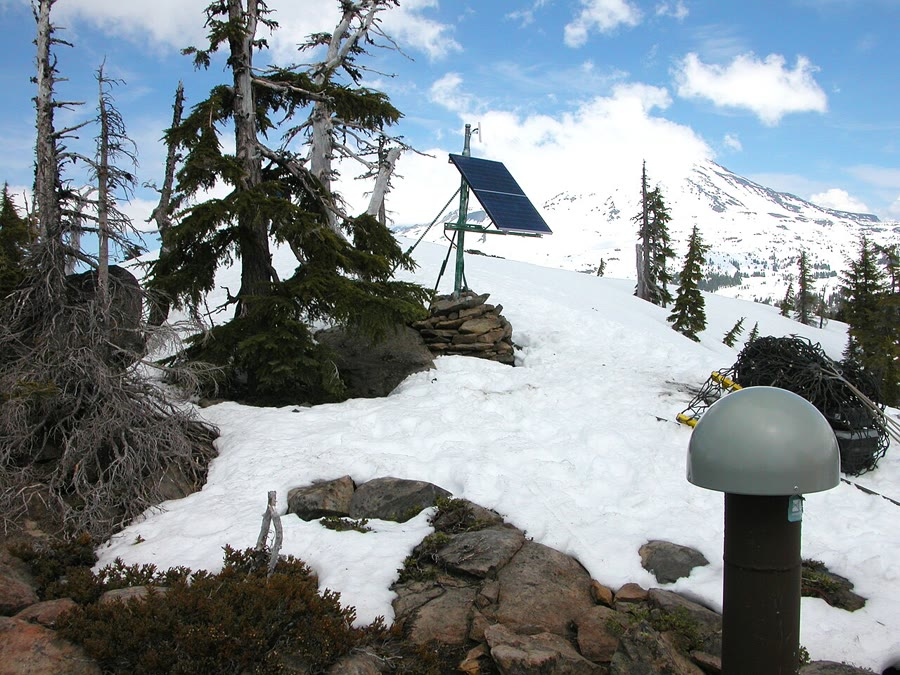
\includegraphics[width=0.62\linewidth]{images/book2/g11-usgs-gps-station.jpg}

{\small Stasiun penentuan posisi dengan satelit yang permanen di sebuah gunung
api di Pegunungan Cascade, Oregon (2007). Antenanya terletak di bawah kubah
kelabu, pada tiang yang tertanam kuat di tanah; panel surya di belakangnya
memberi daya kepada penerimanya. Stasiun seperti itu merekam posisinya sendiri
hari demi hari. Foto: Dave Sherrod, USGS (domain publik).}
\end{omfigure}
% ledger: photo:g11-gps-station

\section{Lempeng kaku pada bola}

Gempa bumi tidak tersebar secara acak di seluruh Bumi: hampir semuanya terjadi
di sepanjang sabuk-sabuk yang sempit, yaitu batas lempeng (Buku 1, kelas 7). Di
dalam lempeng, batuan hampir tidak pecah sama sekali. Karena itu lempeng bukanlah
kulit lunak yang meregang dan berkerut ketika bergerak, melainkan potongan
\omterm{def:g11:lithosphere-asthenosphere:lithosphere}{litosfer} yang kaku yang bergerak sebagai satu kesatuan.

\begin{definition}[Lempeng kaku]\label{def:g11:plate-motions:rigid-plate}
Yang disebut \emph{lempeng kaku}\index{lempeng kaku} adalah potongan \omterm{def:g11:lithosphere-asthenosphere:lithosphere}{litosfer}
yang bergerak sebagai satu blok: jarak antara titik-titik di atasnya tidak
berubah, dan deformasinya terkumpul di zona-zona sempit di sepanjang batasnya.
\end{definition}

Model \omterm{def:g11:plate-motions:rigid-plate}{lempeng kaku} adalah sebuah pendekatan. Beberapa wilayah berdeformasi
sepanjang ratusan kilometer, seperti dataran tinggi di belakang Himalaya atau
bagian barat Amerika Utara, dan model itu memperlakukannya sebagai batas yang
lebar. Tetapi di sebagian besar permukaan Bumi model itu bekerja dengan sangat
baik: kecepatan yang diramalkannya untuk lempeng-lempeng kaku sesuai dengan
kecepatan yang diukur stasiun satelit sampai beberapa milimeter setahun
(\cref{sec:g11:plate-motions:predictive}), sedangkan lempeng-lempeng bergerak
relatif satu sama lain beberapa sentimeter setahun.

Bagaimana sebuah tudung yang kaku dapat bergerak di permukaan bola? Tudung itu
tidak dapat bergeser pada garis lurus, karena garis lurus meninggalkan bola.
Apa pun gerak tudung yang kaku, gerak itu adalah \emph{rotasi} terhadap sumbu
yang melalui pusat Bumi. Sumbu itu memotong permukaan di \emph{kutub rotasi}
lempeng itu. Sebuah titik pada lempeng bergerak di sepanjang lingkaran kecil di
sekeliling kutub itu, dan makin jauh titik itu dari kutub, makin besar
lingkarannya dan makin cepat geraknya (gambar di bawah). Bukti bahwa setiap
gerak tudung yang kaku adalah rotasi seperti itu, dan penggunaan kutub rotasi
untuk memerikan batas lempeng, termasuk dalam Buku~3; di sini hanya
kecepatannya yang digunakan.

\begin{omfigure}
\begin{tikzpicture}[scale=1.15, font=\footnotesize]
  \fill[omSea!45] (0,0) circle (2);
  \draw (0,0) circle (2);
  % small circles about the rotation pole (pole at the top), seen slightly from above
  \foreach \a/\len in {60/0.75, 35/1.23, 0/1.5} {
    \pgfmathsetmacro{\r}{2*cos(\a)}
    \pgfmathsetmacro{\h}{2*sin(\a)}
    \draw[black!45, densely dashed] (-\r,\h) arc[start angle=180, end angle=0, x radius=\r, y radius=0.22*\r];
    \draw[omDef!80!black, line width=0.7pt] (-\r,\h) arc[start angle=180, end angle=360, x radius=\r, y radius=0.22*\r];
    \draw[-{Stealth[length=5pt]}, omProp, line width=1.1pt] (0,\h-0.22*\r) -- ++(\len,0);
  }
  \draw[black!70, dash pattern=on 3pt off 2pt] (0,-2.5) -- (0,2.55);
  \fill (0,2) circle (1.6pt);
  \node[anchor=south west] at (0.05,2.02) {kutub rotasi};
  \node[anchor=north, text=black!70] at (0,-2.5) {sumbu rotasi, melalui pusat};
  \fill (0,0) circle (1pt);
  \node[anchor=west, align=left] at (2.25,0.9) {setiap titik bergerak\\pada lingkaran kecil\\di sekeliling kutub};
  \node[anchor=west, align=left, text=omProp] at (2.25,-0.4) {kecepatan: terbesar\\\ang{90} dari kutub};
\end{tikzpicture}

{\small \omterm{def:g11:plate-motions:rigid-plate}{Lempeng kaku} pada bola berputar terhadap sumbu yang melalui pusat Bumi.
Titik-titik di dekat kutub rotasi bergerak lambat, pada lingkaran-lingkaran
kecil; titik-titik yang berjarak \ang{90} dari kutub bergerak paling cepat
(panah: kecepatan dengan skala sebenarnya).}
\end{omfigure}

Kecepatan sebuah titik mudah dihitung. Titik yang berjarak sudut $\theta$ dari
kutub terletak pada jarak $R\sin\theta$ dari sumbu, dengan $R = \qty{6371}{km}$
jari-jari Bumi. Jika lempeng itu berputar $\omega$ derajat per sejuta tahun,
titik itu menempuh bagian $\omega/360$ dari lingkaran berjari-jari $R\sin\theta$
dalam sejuta tahun:
\[
  v = \frac{\omega}{360} \times 2\pi R\sin\theta
    = \frac{\pi\,\omega}{180}\,R\sin\theta .
\]
Untuk $\omega = \qty{1}{\degree}$ per sejuta tahun dan $\theta = \ang{90}$
hasilnya $\pi \times 6371/180 \approx \qty{111}{km}$ per sejuta tahun,
\qty{11.1}{cm} setahun. Karena itu sebuah lempeng tidak mempunyai satu
kecepatan saja: titik-titiknya bergerak dengan kecepatan yang berkisar dari nol
di kutub rotasi (jika kutub itu terletak pada lempeng) sampai maksimum pada
\ang{90} darinya. Sesar-sesar transform di sepanjang punggung samudra, yang
membuat dua lempeng bergeser saling melewati, mengikuti lingkaran-lingkaran
kecil di sekeliling kutub rotasi relatif kedua lempeng itu.
% ledger: earth:Rmean (shared), nnr56:poles

Kumpulan kutub rotasi yang diterbitkan memberikan, untuk setiap lempeng, letak
kutubnya dan laju putarannya. Salah satunya, yang terutama disusun dari \omterm{def:g11:drift-to-spreading:spreading-rate}{laju
pemekaran} dan arah pemekaran yang diukur di sepanjang punggung-punggung samudra,
memerikan 56 lempeng; lempeng Pasifik berputar
\ang{0.651} per sejuta tahun, lempeng Eurasia \ang{0.223}. Dari angka-angka
itu sebuah komputer menghitung kecepatan setiap titik pada setiap lempeng
(peta di bawah).
% ledger: nnr56:poles, nnr56:data

\begin{omfigure}
\begin{tikzpicture}
\begin{axis}[ommap, width=\linewidth, xtick={-180,-90,...,180}, ytick={-60,0,60}]
\addplot[fill=omLithAlluv, draw=black!45, line width=0.2pt] table {figdata/out/shared-geo-land.dat};
\addplot[omRidge, line width=0.6pt] table {figdata/out/shared-geo-school-ridge.dat};
\addplot[omRidge!70!black, line width=0.6pt] table {figdata/out/shared-geo-school-transform.dat};
\addplot[omTrench, line width=0.6pt] table {figdata/out/shared-geo-school-subduction.dat};
\addplot[fill=omTrench, draw=none] table {figdata/out/shared-geo-school-teeth.dat};
\addplot[black!65, line width=0.6pt] table {figdata/out/shared-geo-school-collision.dat};
% computed in figdata/grade-11/plate_velocities.py (NNR-MORVEL56); 2.5 degrees per cm/yr
\addplot[black, line width=0.8pt, -{Stealth[length=4pt]}, quiver={u=\thisrow{dx}, v=\thisrow{dy}}]
  table[x=lon, y=lat] {figdata/out/grade-11-plate_velocities-arrows.dat};
\addplot[omProp, line width=1.2pt, -{Stealth[length=5pt]}, quiver={u=\thisrow{dx}, v=\thisrow{dy}}]
  table[x=lon, y=lat] {figdata/out/grade-11-plate_velocities-hawaii.dat};
\addplot[only marks, mark=*, mark size=1.3pt, omProp] coordinates {(-155.46,19.80)};
\node[font=\scriptsize, anchor=north, fill=white, fill opacity=0.75, text opacity=1, inner sep=1pt]
  at (axis cs:-150,15) {Mauna Kea};
\draw[black, line width=0.8pt, -{Stealth[length=4pt]}] (axis cs:-172,-80) -- (axis cs:-147,-80);
\node[font=\scriptsize, anchor=west, fill=white, fill opacity=0.75, text opacity=1, inner sep=1pt]
  at (axis cs:-145,-80) {\qty{10}{cm} setahun};
\end{axis}
\end{tikzpicture}

{\small Kecepatan titik-titik di dalam 16 lempeng, yang dihitung dari kutub
rotasinya yang diterbitkan, dalam kerangka acuan yang di dalamnya \omterm{def:g11:lithosphere-asthenosphere:lithosphere}{litosfer}
secara keseluruhan tidak berputar. Lempeng Pasifik, Nazca, Cocos, Australia, dan
India bergerak paling cepat; lempeng Eurasia, Amerika Utara, Amerika Selatan,
dan Antarktika bergerak lambat. Panah merah: lempeng Pasifik di Mauna Kea. Kutub
rotasi: Argus, Gordon, dan DeMets (2011); batas lempeng: Bird (2003); daratan:
Natural Earth.}
\end{omfigure}
% ledger: nnr56:poles, data:pb2002, data:ne-land

\section{Mengukur gerak}

\subsection{Dua cara mengukur kecepatan}

Jalur-jalur magnetik dasar samudra memberikan kecepatan dua lempeng saling
menjauh melintasi punggung samudra (\cref{ch:g11:drift-to-spreading}): bagilah
jarak sebuah jalur dari sumbu punggung dengan umurnya. Kecepatan yang diperoleh
adalah rata-rata sepanjang umur jalur itu, sering kali beberapa juta tahun
terakhir, dan merupakan kecepatan \emph{relatif}, yaitu kecepatan satu lempeng
yang dilihat dari lempeng lainnya. Jalur-jalur itu tidak memberi tahu apa-apa
tentang lempeng-lempeng yang bertemu di palung atau zona tumbukan, karena di
sana tidak terbentuk dasar samudra.

Penentuan posisi dengan satelit mengukur gerak satu titik, pada masa kini,
selama beberapa tahun atau dasawarsa. Stasiun permanen ditambatkan pada batuan
padat, sehingga ia bergerak bersama lempeng; posisi hariannya, bila digambarkan
terhadap waktu, berjajar pada sebuah garis lurus yang kemiringannya adalah
kecepatan stasiun itu.

\begin{method}[Laju dari deret waktu posisi]\label{met:g11:plate-motions:rate}
\begin{enumerate}
  \item Gambarkan posisi timur dan posisi utara stasiun terhadap
        waktu, pada dua grafik atau pada grafik yang sama.
  \item Tarik garis lurus yang paling baik mengikuti setiap deret (atau baca dua
        titik yang berjauhan padanya). Kemiringannya, dalam milimeter per tahun,
        adalah kecepatan timur $v_E$ atau kecepatan utara $v_N$; stasiun yang
        bergerak ke barat atau ke selatan mempunyai kecepatan negatif.
  \item Kecepatan stasiun adalah $v = \sqrt{v_E^2 + v_N^2}$; arahnya
        membentuk sudut $\alpha$ dengan garis timur--barat sehingga
        $\tan\alpha = |v_N|/|v_E|$, ke arah utara jika $v_N > 0$ dan ke arah
        timur jika $v_E > 0$.
\end{enumerate}
\end{method}

\begin{omfigure}
\begin{tikzpicture}
\begin{axis}[ompt, name=a, width=0.5\linewidth, height=5.6cm, xmin=1995, xmax=2027, ymin=-200, ymax=120,
  xlabel={tahun}, ylabel={posisi (\unit{cm})}, xtick={2000,2010,2020},
  xticklabel style={/pgf/number format/set thousands separator={}},
  title={\small Mauna Kea, Hawaii (MKEA)}, tick label style={font=\scriptsize}]
% computed in figdata/grade-11/gnss_series.py; ledger: data:b2-ngl-gnss
\addplot[only marks, mark=*, mark size=0.5pt, omDef] table[x=year, y=north] {figdata/out/grade-11-gnss_series-mkea.dat};
\addplot[only marks, mark=*, mark size=0.5pt, omProp] table[x=year, y=east] {figdata/out/grade-11-gnss_series-mkea.dat};
\node[font=\scriptsize, text=omDef!80!black, anchor=west] at (axis cs:1996.5,80) {utara};
\node[font=\scriptsize, text=omProp!80!black, anchor=west] at (axis cs:1996.5,-120) {timur};
\end{axis}
\begin{axis}[ompt, at={(a.east)}, anchor=west, xshift=0.9cm, width=0.5\linewidth, height=5.6cm, xmin=1995, xmax=2027,
  ymin=-10, ymax=70, xlabel={tahun}, xtick={2000,2010,2020},
  xticklabel style={/pgf/number format/set thousands separator={}},
  title={\small Wettzell, Jerman (WTZR)}, tick label style={font=\scriptsize}]
\addplot[only marks, mark=*, mark size=0.5pt, omDef] table[x=year, y=north] {figdata/out/grade-11-gnss_series-wtzr.dat};
\addplot[only marks, mark=*, mark size=0.5pt, omProp] table[x=year, y=east] {figdata/out/grade-11-gnss_series-wtzr.dat};
\node[font=\scriptsize, text=omDef!80!black, anchor=west] at (axis cs:2014,22) {utara};
\node[font=\scriptsize, text=omProp!80!black, anchor=west] at (axis cs:2006,40) {timur};
\end{axis}
\end{tikzpicture}

{\small Posisi rata-rata bulanan dua stasiun permanen, diukur dari bulan
pertamanya: timur (merah) dan utara (biru). Setiap deret berjajar pada garis
lurus, yang kemiringannya adalah kecepatan stasiun ke arah itu. Mauna Kea, di lempeng Pasifik, bergerak ke barat dan ke utara; Wettzell, di
lempeng Eurasia, ke timur dan ke utara, sekitar tiga kali lebih lambat. Data:
Nevada Geodetic Laboratory (Blewitt, Hammond, dan Kreemer, 2018).}
\end{omfigure}
% ledger: data:b2-ngl-gnss

\begin{example}[Stasiun di Mauna Kea]\label{ex:g11:plate-motions:mkea}
Dari Oktober 1996 sampai September 2026, posisi bulanan stasiun
Mauna Kea mengikuti dua garis lurus dengan kemiringan $v_E =
\qty{-63.2}{mm}$ setahun (ke barat) dan $v_N = \qty{+34.5}{mm}$ setahun.
Kecepatannya $\sqrt{63.2^2 + 34.5^2} \approx \qty{72}{mm}$ setahun, dan $\tan\alpha
= 34.5/63.2 \approx 0.546$ memberikan $\alpha \approx \ang{29}$: stasiun itu
bergerak \qty{7.2}{cm} setahun ke arah \ang{29} di utara arah barat. Kutub
rotasi lempeng Pasifik meramalkan \qty{6.9}{cm} setahun, \ang{28} di utara arah
barat, di tempat ini.
\end{example}
% ledger: data:b2-ngl-gnss, nnr56:poles (prediction computed in plate_velocities.py)

Titik-titiknya tersebar beberapa milimeter di sekitar garis-garis itu, jauh
lebih kecil daripada gerak selama satu tahun: setelah pengukuran beberapa tahun,
kecepatan sebuah stasiun diketahui dengan ketelitian lebih baik daripada satu
milimeter setahun.

\subsection{Gerak relatif dan gerak mutlak}

Kecepatan selalu diukur terhadap sesuatu. Stasiun Mauna Kea bergerak
\qty{7.2}{cm} setahun terhadap kerangka acuan yang terikat pada seluruh Bumi;
dilihat dari stasiun di Amerika Utara, yang juga bergerak, kecepatannya berbeda.

\begin{definition}[Gerak relatif; gerak mutlak]\label{def:g11:plate-motions:relative-motion}
Yang disebut \emph{gerak relatif}\index{gerak relatif} lempeng $A$ terhadap
lempeng $B$ adalah geraknya seperti yang dilihat oleh pengamat yang berdiri di
$B$. Yang disebut \emph{gerak mutlak}\index{gerak mutlak} sebuah lempeng adalah
geraknya terhadap kerangka acuan yang terikat pada bagian dalam Bumi, misalnya
sekumpulan titik panas yang dianggap tetap, atau kerangka acuan yang di dalamnya
\omterm{def:g11:lithosphere-asthenosphere:lithosphere}{litosfer} secara keseluruhan tidak berputar.
\end{definition}

Punggung samudra, palung, dan sesar transform dibentuk oleh \omterm{def:g11:plate-motions:relative-motion}{gerak relatif}: yang
penting di suatu batas adalah bagaimana kedua lempeng bergerak relatif satu sama
lain. Kecepatan relatif dijumlahkan seperti perpindahan yang dihasilkannya.

\begin{proposition}[Kecepatan relatif dijumlahkan seperti panah]\label{prop:g11:plate-motions:sum}
Misalkan $\vec v_{A/B}$ kecepatan lempeng $A$ relatif terhadap lempeng $B$, di
suatu titik pada batasnya, dan demikian pula untuk pasangan-pasangan lainnya.
Untuk setiap tiga lempeng $A$, $B$, $C$,
\[
  \vec v_{A/C} = \vec v_{A/B} + \vec v_{B/C},
  \qquad\text{dan}\qquad
  \vec v_{B/A} = -\vec v_{A/B}.
\]
\end{proposition}

\begin{proof}
Selama waktu singkat $\Delta t$, misalkan sebuah titik yang terikat pada $A$
berpindah dari posisi $P$ ke $P'$ seperti yang dilihat dari $C$, dan titik pada
$B$ yang semula berada di $P$ berpindah ke $Q$ seperti yang dilihat dari $C$.
Dilihat dari $B$, titik pada $A$ itu telah berpindah dari $Q$ ke
$P'$. Perpindahan-perpindahan itu dijumlahkan sebagai vektor:
$\overrightarrow{PP'} = \overrightarrow{PQ} + \overrightarrow{QP'}$, yaitu
perpindahan $A$ dilihat dari $C$ = perpindahan $B$ dilihat dari $C$ +
perpindahan $A$ dilihat dari $B$. Pembagian dengan $\Delta t$ memberikan $\vec v_{A/C}
= \vec v_{B/C} + \vec v_{A/B}$. Dengan $C = A$, ruas kiri bernilai nol: $\vec
v_{B/A} = -\vec v_{A/B}$.
\end{proof}

\begin{method}[Menutup segitiga kecepatan]\label{met:g11:plate-motions:triangle}
\begin{enumerate}
  \item Tuliskan setiap kecepatan yang diketahui dengan komponen timur dan
        utaranya, semuanya diukur di titik yang sama.
  \item Untuk mencari $\vec v_{A/B}$ dari kecepatan $A$ dan $B$ dalam kerangka
        acuan $C$ yang sama, kurangkan: $\vec v_{A/B} = \vec v_{A/C} - \vec v_{B/C}$,
        komponen demi komponen.
  \item Pada gambar, letakkan pangkal $\vec v_{A/C}$ dan $\vec v_{B/C}$ di
        titik yang sama: panah dari ujung $\vec v_{B/C}$ ke ujung
        $\vec v_{A/C}$ adalah $\vec v_{A/B}$, dan panah itu menutup segitiganya.
  \item Hitung panjang dan arahnya seperti pada
        \cref{met:g11:plate-motions:rate}.
\end{enumerate}
\end{method}

\begin{example}[Sesar San Andreas]\label{ex:g11:plate-motions:san-andreas}
Di California tengah, pada \ang{35.5} LU dan \ang{120.5} BB, kutub-kutub
rotasi memberikan kecepatan $(-42.1, +26.4)$ kepada lempeng Pasifik dan
$(-11.9, -14.8)$ kepada lempeng Amerika Utara, dalam milimeter setahun (timur,
utara), dalam kerangka acuan seluruh \omterm{def:g11:lithosphere-asthenosphere:lithosphere}{litosfer}. Lempeng Pasifik relatif terhadap
Amerika Utara bergerak dengan $(-42.1 + 11.9,\ 26.4 + 14.8) = (-30.2, +41.2)$,
yaitu $\sqrt{30.2^2 + 41.2^2} \approx \qty{51}{mm}$ setahun, ke arah
\ang{36} di barat arah utara (gambar di bawah). Sesar San
Andreas, yang membentang ke arah barat laut, menampung sebagian besar
pergeseran ini.
\end{example}
% ledger: nnr56:poles (computed in plate_velocities.py: relative pa/na at 120.5 W 35.5 N)

\begin{omfigure}
\begin{tikzpicture}[x=0.065cm, y=0.065cm, font=\footnotesize]
  % mm/yr, from plate_velocities.py: PA (-42.1, 26.4), NA (-11.9, -14.8), PA/NA (-30.2, 41.2)
  \draw[black!25] (-8,0) -- (8,0) (0,-8) -- (0,8);
  \draw[-{Stealth[length=5pt]}, omProp, line width=1.1pt] (0,0) -- (-42.1,26.4)
    node[pos=0.55, above right, inner sep=1pt] {$\vec v_{\mathrm{PA}}$};
  \draw[-{Stealth[length=5pt]}, omDef, line width=1.1pt] (0,0) -- (-11.9,-14.8)
    node[pos=0.8, right=2pt] {$\vec v_{\mathrm{NA}}$};
  \draw[-{Stealth[length=5pt]}, black, line width=1.1pt] (-11.9,-14.8) -- (-42.1,26.4)
    node[pos=0.4, left=9pt, align=right] {$\vec v_{\mathrm{PA/NA}}$\\\qty{51}{mm} setahun};
  \fill (0,0) circle (0.9pt);
  % compass
  \draw[-{Stealth[length=4pt]}] (25,10) -- (25,24) node[above] {U};
  \draw[-{Stealth[length=4pt]}] (25,10) -- (39,10) node[right] {T};
  \draw (25,-18) -- (40.4,-18);
  \node[below] at (32.7,-18) {\qty{20}{mm} setahun};
  \draw (25,-17) -- (25,-19) (40.4,-17) -- (40.4,-19);
\end{tikzpicture}

{\small Menutup segitiga kecepatan di California tengah (dengan skala
sebenarnya). Merah: lempeng Pasifik; biru: lempeng Amerika Utara, keduanya dalam
kerangka acuan seluruh \omterm{def:g11:lithosphere-asthenosphere:lithosphere}{litosfer}. Hitam: lempeng Pasifik dilihat dari Amerika
Utara, panah dari ujung panah biru ke ujung panah merah.}
\end{omfigure}

\section{Jejak titik panas}

\subsection{Lempeng di atas gumpalan yang tetap}

Hawaii terletak di tengah lempeng Pasifik, lebih dari \qty{3000}{km}
dari batas lempeng yang terdekat.
% ledger: usgs:hawaii-hotspot (Book 1 row)
 Gunung-gunung apinya dipasok oleh sebuah titik panas (Buku~1,
kelas~7). Lempeng bergerak di atasnya, dan setiap gunung api terbawa menjauhi
titik panas itu sementara gunung api baru tumbuh di belakangnya.

\begin{definition}[Jejak titik panas]\label{def:g11:plate-motions:hotspot-track}
Yang disebut \emph{jejak titik panas}\index{jejak titik panas} adalah deretan
gunung api, dan gunung api tenggelam yang disebut gunung bawah laut, yang dibawa
lempeng menjauhi titik panas ketika lempeng itu bergerak di atasnya: gunung api
yang aktif berdiri di atas titik panas, dan gunung-gunung api makin tua seiring
jaraknya dari titik panas itu.
\end{definition}

\begin{omfigure}
\begin{tikzpicture}[font=\footnotesize]
  % plate moving to the left over a fixed plume (not to scale)
  \fill[omSea!50] (0,0) rectangle (11,0.9);
  \fill[black!22] (0,-0.9) rectangle (11,0);
  \draw (0,0) -- (11,0);
  \draw[densely dashed] (0,0.9) -- (11,0.9) node[right] {permukaan laut};
  \node[anchor=east] at (10.95,-0.45) {litosfer};
  \fill[omLithPeridotite!40] (0,-2.3) rectangle (11,-0.9);
  \node[anchor=west] at (0.1,-1.6) {astenosfer};
  % plume
  \fill[omProp!55] (8.6,-2.3) -- (8.6,-1.2) .. controls (8.6,-0.9) and (9.2,-0.9) .. (9.2,-1.2) -- (9.2,-2.3) -- cycle;
  \fill[omProp!55] (8.75,-0.95) rectangle (9.05,0);
  \node[anchor=north, align=center] at (8.9,-2.35) {gumpalan, tetap di mantel};
  % volcanoes: active over the plume, older ones carried left, eroded and sunk
  \fill[black!65] (8.0,0) -- (8.9,1.6) -- (9.8,0) -- cycle;
  \fill[black!55] (5.4,0) -- (6.2,1.15) -- (7.0,0) -- cycle;
  \fill[black!50] (3.0,0) -- (3.55,0.62) -- (3.85,0.62) -- (4.4,0) -- cycle;
  \fill[black!45] (0.8,0) -- (1.25,0.42) -- (1.65,0.42) -- (2.1,0) -- cycle;
  \node[above] at (8.9,1.6) {aktif};
  \node[above] at (6.2,1.15) {$t_1$};
  \node[above] at (3.7,0.62) {$t_2$};
  \node[above] at (1.45,0.42) {$t_3$};
  % plate motion
  \draw[-{Stealth[length=6pt]}, line width=1.2pt] (6.5,-0.45) -- (4.0,-0.45) node[left] {lempeng bergerak, kecepatan $v$};
  % distance d = v t
  \draw[{Stealth[length=4pt]}-{Stealth[length=4pt]}] (3.7,2.3) -- (8.9,2.3) node[midway, above] {$d_2 = v\,t_2$};
  \draw[black!50] (3.7,1.05) -- (3.7,2.4) (8.9,2.0) -- (8.9,2.4);
\end{tikzpicture}

{\small Lempeng yang bergerak dengan kecepatan $v$ di atas gumpalan yang tetap
di mantel (tidak berskala). Gunung api berumur $t$, yang dibangun di atas
gumpalan itu, telah terbawa sejauh $d = v\,t$; gunung-gunung api yang lebih tua
tererosi dan tenggelam di bawah laut.}
\end{omfigure}

\begin{proposition}[Kecepatan dari jejak titik panas]\label{prop:g11:plate-motions:hotspot}
Jika titik panas tetap di tempatnya di mantel dalam dan lempeng di atasnya
bergerak dengan kecepatan tetap $v$ ke arah yang tetap, gunung api yang berdiri
di atas titik panas pada waktu $t$ yang lalu kini terletak pada jarak
\[
  d = v\,t
\]
dari gunung api yang aktif, di sepanjang jejak itu. Umur gunung-gunung api, bila
digambarkan terhadap jaraknya, terletak pada sebuah garis lurus melalui titik
asal yang kemiringannya $1/v$, dan $v$ adalah kecepatan mutlak lempeng itu.
\end{proposition}

\begin{proof}
Gunung api itu dibangun di tempat lempeng berada di atas titik panas, dan sejak
itu ia bergerak bersama lempeng. Selama waktu $t$ lempeng telah berpindah sejauh
$v\,t$ ke arah yang tetap, sehingga gunung api itu terletak pada jarak itu dari
titik lempeng yang sekarang berada di atas titik panas, tempat gunung api yang
aktif berdiri. Hubungan $t = d/v$ adalah persamaan garis lurus melalui titik
asal dengan kemiringan $1/v$. Kecepatan itu diukur terhadap titik panas, yaitu
terhadap mantel dalam: kecepatan itu adalah kecepatan mutlak.
\end{proof}

\subsection{Rantai Hawaii--Emperor}

Dari Pulau Hawaii, sederet pulau, terumbu, dan gunung bawah laut membentang
sekitar \qty{3400}{km} ke arah barat-barat laut, lalu berbelok tajam dan
berlanjut ke utara sebagai gunung-gunung bawah laut Emperor, dengan gunung bawah
laut Suiko saja terletak \qty{4860}{km} dari Kilauea, sampai ke palung-palung di
lepas pantai Kamchatka dan Kepulauan Aleut (citra di bawah).
% ledger: cd87:ages

\begin{omfigure}
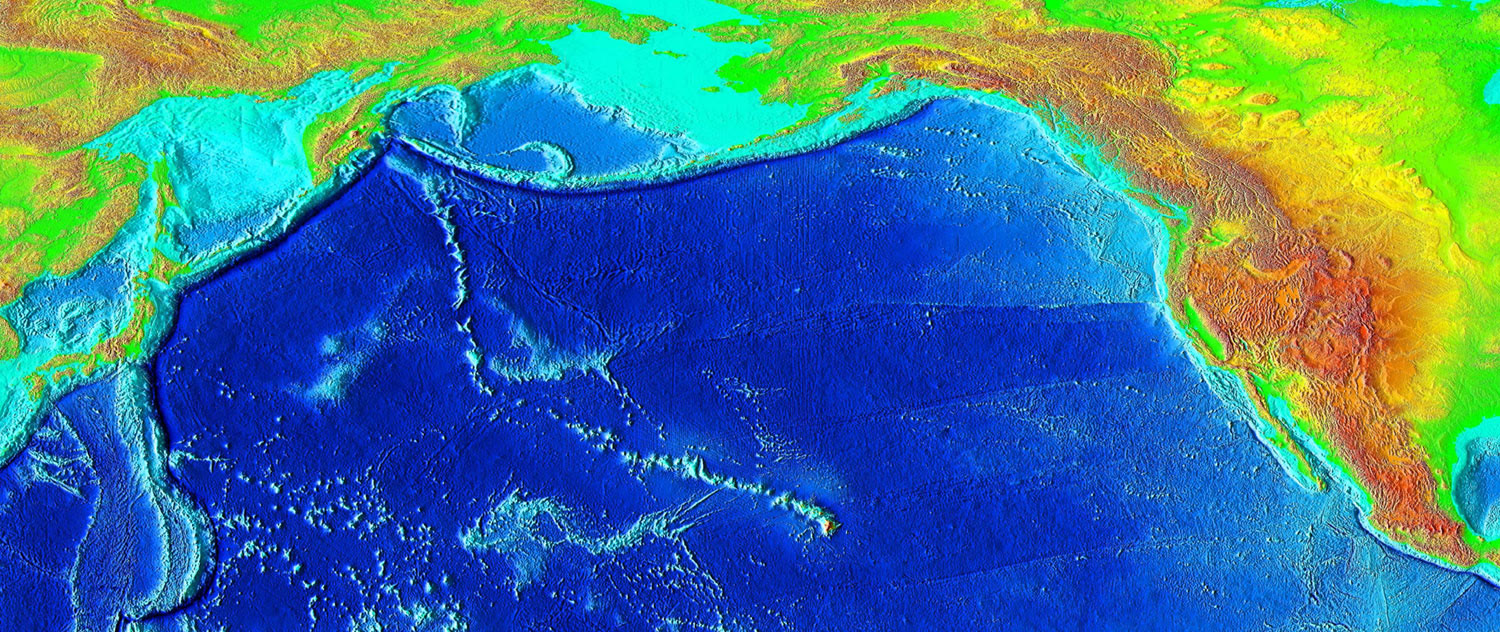
\includegraphics[width=\linewidth]{images/book2/g11-ngdc-hawaii-chain.jpg}

{\small Relief berbayang dasar Pasifik Utara. Rantai Hawaii membentang dari
Pulau Hawaii (tengah bawah, cokelat) ke arah barat-barat laut; di tikungan,
rantai itu berbelok ke utara menjadi gunung-gunung bawah laut Emperor, yang
berakhir di palung di sepanjang Kamchatka dan Kepulauan Aleut. Citra: National
Geophysical Data Center, NOAA (domain publik).}
\end{omfigure}
% ledger: photo:g11-hawaii-chain

Penanggalan kalium--argon lava dari 37 gunung api rantai itu, yang dikumpulkan di
pulau-pulau, dikeruk dari gunung-gunung bawah laut, atau dibor menembus
sedimennya, memberikan umurnya (grafik di bawah). Mauna Kea berumur sekitar
\num{0.4} juta tahun, Kauai \num{5.1}, Midway \num{27.7}, dan gunung bawah laut
Suiko, di dekat ujung jauh rantai Emperor, \num{64.7}. Umur-umur itu bertambah
seiring jaraknya dari Kilauea, gunung api yang aktif, seperti yang diramalkan
oleh \omterm{def:g11:plate-motions:hotspot-track}{jejak titik panas}.
% ledger: cd87:ages

\begin{omfigure}
\begin{tikzpicture}
\begin{axis}[ompt, width=0.82\linewidth, height=6.4cm, xmin=0, xmax=5000, ymin=0, ymax=70,
  xlabel={jarak dari Kilauea di sepanjang rantai (\unit{km})}, ylabel={umur (juta tahun)},
  xticklabel style={/pgf/number format/set thousands separator={}},
  legend style={font=\scriptsize, at={(0.03,0.97)}, anchor=north west}, legend cell align=left]
% computed in figdata/grade-11/hawaii_chain.py; ledger: cd87:ages
\addplot[only marks, mark=o, mark size=1.6pt, omDef, error bars/.cd, y dir=both, y explicit]
  table[x=dist, y=age, y error=err] {figdata/out/grade-11-hawaii_chain-hawaiian.dat};
\addplot[only marks, mark=triangle, mark size=2pt, omProp, error bars/.cd, y dir=both, y explicit]
  table[x=dist, y=age, y error=err] {figdata/out/grade-11-hawaii_chain-emperor.dat};
\addplot[black, densely dashed, line width=0.6pt] table[x=dist, y=age] {figdata/out/grade-11-hawaii_chain-fit.dat};
\legend{rantai Hawaii, tikungan dan rantai Emperor, {garis melalui titik asal, \qty{9.1}{cm} setahun}}
\draw[black!50, densely dotted] (axis cs:3400,0) -- (axis cs:3400,70);
\node[font=\scriptsize, anchor=south, rotate=90] at (axis cs:3400,8) {tikungan};
\node[font=\scriptsize, anchor=north west] at (axis cs:519,5.1) {Kauai};
\node[font=\scriptsize, anchor=south] at (axis cs:2432,30) {Midway};
\node[font=\scriptsize, anchor=south east] at (axis cs:4860,65.5) {Suiko};
\end{axis}
\end{tikzpicture}

{\small Umur gunung-gunung api rantai Hawaii--Emperor terhadap jaraknya dari
Kilauea, dengan ketidakpastian umurnya. Di sepanjang rantai Hawaii titik-titiknya
mengikuti garis lurus melalui titik asal; di luar tikungan umurnya bertambah
lebih cepat seiring jarak. Data: Clague dan Dalrymple
(1987).}
\end{omfigure}

Di sepanjang rantai Hawaii, sampai sekitar \qty{3300}{km}, titik-titiknya
tersebar di sekitar garis lurus melalui titik asal. Garis yang paling cocok
dengan 26 gunung api bertanggal pada bagian ini naik satu juta tahun setiap
\qty{91}{km}: menurut \cref{prop:g11:plate-motions:hotspot}, lempeng Pasifik
telah bergerak di atas titik panas dengan kecepatan sekitar \qty{91}{km} per
sejuta tahun, \qty{9.1}{cm} setahun. Para penyusun data umur itu, yang mencocokkan
seluruh rantai dengan cara mereka sendiri, mendapatkan \qty{8.6}{cm} setahun.
% ledger: cd87:ages (fit computed in hawaii_chain.py), cd87:rate

Di luar tikungan, umurnya bertambah lebih cepat seiring jarak: di sepanjang
rantai Emperor lempeng bergerak lebih lambat, rata-rata sekitar \qty{6.5}{cm}
setahun (garis lurus terbaik melalui sembilan gunung bawah laut yang bertanggal).
Dan rantai itu berubah arah. Jika titik panas tetap di tempatnya, tikungan itu
merekam perubahan arah gerak lempeng Pasifik. Penanggalan yang lebih baru
menempatkan awal tikungan itu di dekat gunung bawah laut Kimmei, sekitar 50 juta
tahun yang lalu, pada waktu yang sama dengan penataan ulang punggung-punggung
pemekaran di Pasifik dan gunung api pertama busur-busur kepulauan di sepanjang
tepi baratnya: lempeng itu berganti haluan.
% ledger: cd87:ages (Emperor fit computed in hawaii_chain.py), sc06:bend

\section{Daya ramal model}\label{sec:g11:plate-motions:predictive}

Model lempeng menyatakan bahwa beberapa \omterm{def:g11:plate-motions:rigid-plate}{lempeng kaku} berputar terhadap kutub
rotasinya, dan bahwa hampir segala sesuatu terjadi di batas-batasnya.
Kekuatannya adalah bahwa pengukuran dengan metode yang sama sekali berbeda,
dalam rentang waktu yang sangat berbeda, memberikan jawaban yang sama.

\begin{itemize}
  \item \emph{Gempa bumi dan gunung api} berkumpul di sepanjang batas, dan jenis
        batas meramalkan jenisnya: gempa bumi dangkal di sepanjang punggung
        samudra, gempa bumi dalam hanya di dekat palung (\cref{ch:g11:subduction-zones}).
  \item \emph{Dasar samudra} paling muda di sepanjang punggung samudra dan makin
        tua seiring jaraknya dari punggung, secara simetris di kedua sisi
        (\cref{ch:g11:drift-to-spreading}).
  \item \emph{Sabuk pegunungan} terangkat di tempat lempeng-lempeng menumbuk:
        India masih bergerak ke arah Eurasia dengan kecepatan sekitar
        \qty{4.5}{cm} setahun melintasi Himalaya, seperti yang dihitung dari
        kutub-kutub rotasi (\cref{ch:g12:mountain-building}).
  \item \emph{Kecepatan sesuai di antara berbagai metode}: tabel di bawah
        membandingkan kecepatan yang diukur sekarang dengan penentuan posisi
        dengan satelit dengan kecepatan yang diramalkan oleh kutub-kutub
        rotasi, yang \omterm{def:g11:drift-to-spreading:spreading-rate}{laju pemekarannya} terutama berasal dari jalur-jalur
        magnetik dan merata-ratakan gerak selama \num{0.8} sampai \num{3.2}
        juta tahun terakhir, dan dengan kecepatan yang direkam oleh \omterm{def:g11:plate-motions:hotspot-track}{jejak titik
        panas} selama puluhan juta tahun.
\end{itemize}
% ledger: nnr56:poles, nnr56:data (India-Eurasia computed in plate_velocities.py at 85 E 28 N)

\begin{center}
\small
\begin{tabular}{|l|c|c|}
\hline
yang diukur & metode & kecepatan (\unit{cm} setahun) \\ \hline
Mauna Kea, lempeng Pasifik & posisi satelit, 30 tahun & 7.2 \\
Mauna Kea, lempeng Pasifik & kutub rotasi & 6.9 \\
Wettzell, lempeng Eurasia & posisi satelit, 31 tahun & 2.6 \\
Wettzell, lempeng Eurasia & kutub rotasi & 2.3 \\
lempeng Pasifik di atas titik panas Hawaii & umur gunung api, 40 juta tahun & 9.1 \\ \hline
\end{tabular}
\end{center}
% ledger: data:b2-ngl-gnss, nnr56:poles, cd87:ages (all computed in figdata/grade-11)

Kecepatan dari kutub rotasi dan kecepatan stasiun sesuai sampai
\qty{0.3}{cm} setahun, meskipun yang pertama merata-ratakan jutaan tahun dan
yang kedua hanya beberapa dasawarsa: lempeng-lempeng bergerak sekarang seperti
gerakannya selama jutaan tahun. Kecepatan dari titik panas lebih besar:
kecepatan itu diukur dalam kerangka acuan lain, yaitu kerangka titik panas itu
sendiri, dan selama waktu yang jauh lebih panjang.

Satu pola lagi muncul bila kecepatan seluruh lempeng dibandingkan. Lempeng-lempeng
yang bergerak paling cepat, yaitu Cocos, Nazca, Pasifik, Australia, dan Laut
Filipina, semuanya mempunyai tepi panjang yang tenggelam ke dalam mantel di
sebuah palung; kecepatan rata-ratanya sekitar \qty{6.5}{cm} setahun.
Lempeng-lempeng yang tidak mempunyai tepi seperti itu, di antaranya lempeng
Eurasia, Amerika Utara, Amerika Selatan, Afrika, dan Antarktika, bergerak
rata-rata sekitar \qty{2.4}{cm} setahun. Petunjuk tentang penggerak lempeng ini
dibahas lagi pada \cref{ch:g11:subduction-zones}.
% ledger: nnr56:rms (means computed in plate_velocities.py)

\section{Latihan}

\begin{exercise}[$\star$]\label{exo:g11:plate-motions:1}
Definisikan \omterm{def:g11:plate-motions:rigid-plate}{lempeng kaku}. Di mana deformasi \omterm{def:g11:lithosphere-asthenosphere:lithosphere}{litosfer} terkumpul, dan pengamatan
seismik sehari-hari apa yang menunjukkannya?
\end{exercise}

\begin{exercise}[$\star$]\label{exo:g11:plate-motions:2}
Stasiun Mauna Kea bergerak \qty{72}{mm} setahun. Nyatakan kecepatan ini dalam
kilometer per sejuta tahun. Berapa jauh stasiun itu bergerak dalam 30 tahun?
Dalam sejuta tahun?
\end{exercise}

\begin{exercise}[$\star$]\label{exo:g11:plate-motions:3}
Dalam sepuluh tahun, sebuah stasiun berpindah \qty{30}{cm} ke timur dan
\qty{40}{cm} ke utara. Tentukan kecepatan timur dan utaranya, kecepatannya, dan
sudut yang dibentuk arahnya dengan arah utara.
\end{exercise}

\begin{exercise}[$\star$]\label{exo:g11:plate-motions:4}
Definisikan \omterm{def:g11:plate-motions:hotspot-track}{jejak titik panas}. Di sepanjang rantai Hawaii, di mana gunung api
yang paling muda, dan ke arah mana umurnya bertambah? Apa yang disampaikan hal
itu tentang arah gerak lempeng Pasifik?
\end{exercise}

\begin{exercise}[$\star$]\label{exo:g11:plate-motions:5}
Kauai terletak \qty{519}{km} dari Kilauea di sepanjang rantai, dan lava
tertuanya berumur \num{5.1} juta tahun. Dengan menganggap titik panas itu tetap,
berapa kecepatan rata-rata lempeng yang membawanya, dalam kilometer per sejuta
tahun dan dalam sentimeter setahun?
\end{exercise}

\begin{exercise}[$\star\star$]\label{exo:g11:plate-motions:6}
Pada grafik kedua deret stasiun, stasiun Wettzell berpindah sekitar
\qty{63}{cm} ke timur dan \qty{48}{cm} ke utara dalam 31 tahun. Tentukan
kecepatan timur dan utaranya, kecepatannya, dan arahnya. Bandingkan kecepatannya
dengan kecepatan Mauna Kea.
\end{exercise}

\begin{exercise}[$\star\star$]\label{exo:g11:plate-motions:7}
Di Islandia, pada \ang{64.5} LU dan \ang{18} BB, kutub-kutub rotasi memberikan
kecepatan $(-10.5, +20.6)$ kepada lempeng Amerika Utara dan $(+7.7, +16.3)$
kepada lempeng Eurasia, dalam milimeter setahun (timur, utara). (1) Tentukan
kecepatan Amerika Utara relatif terhadap Eurasia, besarnya, dan arahnya.
(2) Apa arti kecepatan ini bagi punggung samudra yang melintasi Islandia?
(3) Bandingkan dengan laju \qty{2}{cm} setahun yang sering disebut untuk
Atlantik Utara.
\end{exercise}

\begin{exercise}[$\star\star$]\label{exo:g11:plate-motions:8}
Lempeng Pasifik berputar \ang{0.651} per sejuta tahun. (1) Tentukan kecepatan
titik yang berjarak \ang{90} dari kutub rotasinya, dalam sentimeter setahun.
(2) Bagaimana dengan titik yang berjarak \ang{30} dari kutub? (3) Di mana pada
sebuah lempeng kecepatannya nol? Dapatkah kecepatan seluruh lempeng diberikan
dengan satu angka?
\end{exercise}

\begin{exercise}[$\star\star$]\label{exo:g11:plate-motions:9}
Di utara Himalaya, pada \ang{28} LU dan \ang{85} BT, kutub-kutub rotasi
memberikan kecepatan $(+40.6, +38.6)$ kepada lempeng India dan
$(+24.0, -3.3)$ kepada lempeng Eurasia, dalam milimeter setahun (timur, utara).
(1) Tentukan kecepatan India relatif terhadap Eurasia, besarnya, dan arahnya.
(2) Jika kecepatan itu tetap, berapa jauh kedua lempeng itu akan saling
mendekat dalam 10 juta tahun?
\end{exercise}

\begin{exercise}[$\star\star$]\label{exo:g11:plate-motions:10}
Necker terletak \qty{1058}{km} dari Kilauea dan berumur \num{10.3} juta tahun;
Midway terletak \qty{2432}{km} dari Kilauea dan berumur \num{27.7} juta tahun.
Tentukan kecepatan lempeng di atas titik panas di antara waktu pembentukan kedua
gunung api itu. Bandingkan dengan \qty{9.1}{cm} setahun.
\end{exercise}

\begin{exercise}[$\star\star$]\label{exo:g11:plate-motions:11}
Di suatu titik, lempeng $A$ bergerak \qty{3}{cm} setahun ke timur relatif
terhadap lempeng $B$, dan lempeng $B$ bergerak \qty{4}{cm} setahun ke utara
relatif terhadap lempeng $C$.
(1) Gambarlah segitiga kecepatannya dan tentukan kecepatan $A$ relatif terhadap
$C$: besar dan arahnya. (2) Berapa kecepatan $C$ relatif terhadap $A$?
\end{exercise}

\begin{exercise}[$\star\star\star$]\label{exo:g11:plate-motions:12}
Mauna Kea terletak \qty{54}{km} dari Kilauea dan berumur \num{0.375} juta
tahun. (1) Kecepatan berapa yang diberikannya untuk lempeng itu? (2) Sebuah
gunung api berdiameter beberapa puluh kilometer, dan tumbuh selama beberapa
ratus ribu tahun. Misalkan jaraknya dari titik panas mempunyai ketidakpastian
\qty{25}{km}: di antara nilai-nilai berapa kecepatannya kemudian terletak?
(3) Jelaskan mengapa gunung api muda yang dekat dengan titik panas memberikan
taksiran kecepatan yang buruk, dan mengapa gunung api yang jauh darinya lebih
baik.
\end{exercise}

\begin{exercise}[$\star\star\star$]\label{exo:g11:plate-motions:13}
Posisi bulanan sebuah stasiun tersebar sekitar \qty{5}{mm} di sekitar garis
lurusnya. Sebuah gerak tampak jelas setelah melampaui sepuluh kali sebaran itu.
(1) Berapa lama orang harus mengukur untuk melihat dengan jelas gerak stasiun
Mauna Kea, \qty{72}{mm} setahun? (2) Bagaimana dengan gerak \qty{5}{mm}
setahun, seperti melintasi wilayah yang berdeformasi perlahan di dalam benua?
(3) Mengapa kecepatan lempeng diukur dari jalur-jalur magnetik jauh sebelum
satelit dapat mengukurnya?
\end{exercise}

\begin{exercise}[$\star\star\star$]\label{exo:g11:plate-motions:14}
Di Punggung Tengah Atlantik pada \ang{30} LS (\ang{13.5} BB), kutub-kutub
rotasi memberikan kecepatan $(-4.9, +11.0)$ kepada lempeng Amerika Selatan dan
$(+27.1, +17.9)$ kepada lempeng Afrika, dalam milimeter setahun (timur, utara).
(1) Tentukan kecepatan Amerika Selatan relatif terhadap Afrika, besarnya, dan
arahnya. (2) Simpulkan \omterm{def:g11:drift-to-spreading:spreading-rate}{laju pemekaran penuh} dan laju setengah pemekaran
punggung itu. (3) Sedimen Atlantik Selatan memberikan laju setengah sekitar
\qty{1.9}{cm} setahun yang dirata-ratakan selama 66 juta tahun terakhir
(\cref{ch:g11:drift-to-spreading}). Bandingkan, dan kemukakan apa kiranya arti
perbedaan itu.
\end{exercise}

\begin{exercise}[$\star\star\star$]\label{exo:g11:plate-motions:15}
Sebuah stasiun bergerak tetap \qty{20}{mm} setahun ke timur. Tepat di tengah
sepuluh tahun pengukuran, sebuah gempa bumi menggesernya secara mendadak sejauh
\qty{50}{mm} ke arah barat. (1) Buatlah sketsa posisi timurnya terhadap waktu.
(2) Kecepatan berapa yang akan diperoleh dari posisi pertama dan terakhir saja?
(3) Kecepatan berapa yang diberikan oleh masing-masing paruh deret itu secara
terpisah? (4) Bagaimana seharusnya ahli \omterm{def:g10:measuring-the-earth:geodesy}{geodesi} menangani lompatan seperti itu?
\end{exercise}

\section{Soal: Membaca Rantai Hawaii--Emperor}

\begin{problem}[{Soal akhir pekan --- kecepatan lempeng yang tertulis pada gunung-gunung api}]
\label{pb:g11:plate-motions:1}
% values from Clague and Dalrymple 1987, Table 1.4 (ledger cd87:ages); fits computed in
% figdata/grade-11/hawaii_chain.py (v_hawaiian 91.2, v_emperor_free 64.6); bend sc06:bend;
% MKEA rates data:b2-ngl-gnss
Tabel ini memberikan jarak dari Kilauea, diukur di sepanjang rantai, dan umur
kalium--argon tiga belas gunung api rantai Hawaii--Emperor. Kilauea adalah
gunung api aktif di atas titik panas; tikungan terletak di antara Abbott
dan Daikakuji.

\begin{center}
\small
\begin{tabular}{|l|c|c||l|c|c|}
\hline
gunung api & jarak (\unit{km}) & umur (\unit{Ma}) & gunung api & jarak (\unit{km}) & umur (\unit{Ma}) \\ \hline
Mauna Kea & 54 & 0.375 & Abbott & 3280 & 38.7 \\ \hline
Kauai & 519 & 5.1 & Daikakuji & 3493 & 42.4 \\ \hline
Nihoa & 780 & 7.2 & Koko (selatan) & 3758 & 48.1 \\ \hline
Necker & 1058 & 10.3 & Ojin & 4102 & 55.2 \\ \hline
Laysan & 1818 & 19.9 & Nintoku & 4452 & 56.2 \\ \hline
Midway & 2432 & 27.7 & Suiko (tengah) & 4860 & 64.7 \\ \hline
Colahan & 3128 & 38.6 & & & \\ \hline
\end{tabular}
\end{center}

\medskip
\noindent\textbf{Bagian I --- Umur dan jarak.}
\begin{enumerate}
  \item Gunung api mana di tabel itu yang paling muda, dan mana yang paling
        tua? Bagaimana umurnya berubah di sepanjang rantai?
  \item Tunjukkan bahwa jarak dalam kilometer dibagi umur dalam juta tahun
        adalah kecepatan dalam milimeter setahun.
  \item Hitung kecepatan rata-rata $d/t$ yang diberikan oleh Kauai.
  \item Hitung $d/t$ untuk Necker, Laysan, Midway, Colahan, dan Abbott.
  \item Gambarkan umur terhadap jarak untuk delapan gunung api pada tabel
        yang terletak sebelum tikungan. Apakah titik-titiknya terletak dekat
        dengan garis lurus melalui titik asal?
\end{enumerate}

\medskip
\noindent\textbf{Bagian II --- Kecepatan lempeng di atas titik panas.}
\begin{enumerate}[resume]
  \item Jelaskan mengapa, untuk titik panas yang tetap dan lempeng yang bergerak
        dengan kecepatan tetap $v$, umur $t$ dan jarak $d$ memenuhi $t = d/v$.
  \item Hitung rata-rata kelima kecepatan pada pertanyaan~4.
  \item Garis lurus melalui titik asal yang paling cocok dengan ke-26 gunung
        api bertanggal pada rantai Hawaii memberikan \qty{91}{km} per sejuta
        tahun. Bandingkan dengan pertanyaan~7.
  \item Dengan kecepatan ini, berapa lama lempeng itu membawa Kauai dari titik
        panas ke tempatnya sekarang? Bandingkan dengan umurnya.
  \item Ke arah mana lempeng Pasifik bergerak di atas titik panas itu?
\end{enumerate}

\medskip
\noindent\textbf{Bagian III --- Tikungan.}
\begin{enumerate}[resume]
  \item Hitung kecepatan rata-rata lempeng di antara waktu pembentukan Daikakuji
        dan Suiko (tengah).
  \item Garis lurus terbaik melalui sembilan gunung api bertanggal mulai dari
        Daikakuji memberikan \qty{65}{km} per sejuta tahun. Bandingkan dengan
        kecepatan di sepanjang rantai Hawaii.
  \item Penanggalan yang lebih baru menempatkan awal tikungan di dekat gunung
        bawah laut Kimmei, \qty{3668}{km} dari Kilauea, sekitar 50 juta tahun
        yang lalu. Kecepatan rata-rata berapa yang diberikannya untuk seluruh
        rantai Hawaii? Bandingkan dengan \qty{91}{km} per sejuta tahun, dan
        jelaskan mengapa keduanya dapat sama-sama benar.
  \item Jika titik panas itu tetap, apa yang direkam tikungan itu tentang
        lempeng Pasifik?
  \item Penanggalan yang lebih baru menemukan perubahan kecepatan yang besar di
        sepanjang rantai Emperor dengan sedikit perubahan arah. Jelaskan mengapa
        arah sebuah rantai dan jarak antarumurnya adalah dua keterangan yang
        saling bebas.
\end{enumerate}

\medskip
\noindent\textbf{Bagian IV --- Perbandingan dengan pengukuran satelit masa kini.}
\begin{enumerate}[resume]
  \item Stasiun Mauna Kea bergerak $\qty{-63.2}{mm}$ setahun ke timur dan
        $\qty{+34.5}{mm}$ setahun ke utara. Tentukan kecepatan dan arahnya.
  \item Rantai Hawaii membentang dari Kilauea ke arah barat-barat laut. Apakah
        arah stasiun itu sesuai dengannya?
  \item Stasiun itu memberikan \qty{7.2}{cm} setahun, rantai itu \qty{9.1}{cm}
        setahun. Berikan dua alasan mengapa kedua angka itu tidak harus sama.
  \item Dengan \qty{91}{km} per sejuta tahun, berapa lama lempeng itu akan
        membawa Mauna Kea \qty{100}{km} lagi menjauhi titik panas?
  \item Simpulkan: dengan kecepatan berapa lempeng Pasifik telah bergerak di
        atas titik panas Hawaii selama 40 juta tahun terakhir?
\end{enumerate}
\end{problem}
